% These are the lecture notes for my CSCI360 course SPRING 2017
% at John Jay College of Criminal Justice. They are based largely on
% Schneier's Applied Cryptography.

% Feel free to edit these slides and use them for your own courses.
% HOWEVER DO NOT REMOVE THESE LINES!
% Email me at: awood [at] jjay.cuny.edu
% or at: awood [at] gradcenter.cuny.edu


\documentclass{beamer}

\usepackage{tikz}
\usetikzlibrary{calc}

\usepackage{graphicx}
\usepackage{amsmath}
\usepackage{enumerate}
%\usepackage{ntheorem}
%\usepackage[margin=1in]{geometry}
\usepackage{amssymb}
\usepackage{pdfpages}
%\usepackage{mathtools}
\usepackage{hyperref}
\usepackage{tikz}
\usepackage{booktabs}

\usepackage{forest}
\usepackage{verbatim}
\usepackage{color}
\usepackage{caption}


\usetikzlibrary{matrix,shapes,arrows,positioning,chains, calc}



\setbeamertemplate{footline}[frame number]
\setbeamertemplate{navigation symbols}{} 

\newtheorem{thm}{Theorem}[section]
\newtheorem{lem}{Lemma}
\newtheorem{cl}{Claim}
\newtheorem{cor}{Corollary}[section]
\newtheorem{conj}{Conjecture}
\newtheorem{quest}{Question}
\newtheorem{defn}{Definition}[section]
\newtheorem{obs}{Observation}[section]
\newtheorem{exam}{Example}

\newcommand{\im}{\operatorname{im}}
\newcommand{\id}{\operatorname{id}}
\newcommand{\interior}{\operatorname{int}}
\newcommand{\bdry}{\operatorname{bdry}}
\newcommand{\<}{\langle}
\renewcommand{\>}{\rangle}
\newcommand{\Gab}{(G_\phi)^{ab}} 
\newcommand{\phibar}{\bar{\phi}}
\newcommand{\Z}{\mathbb{Z}}
\newcommand{\N}{\mathbb{N}}
\newcommand{\Q}{\mathbb{Q}}
\newcommand{\R}{\mathbb{R}}
\newcommand{\C}{\mathbb{C}}
\newcommand{\A}{\mathcal{A}}
\newcommand{\OO}{\mathcal{O}}
\newcommand{\UU}{\mathcal{U}}
\newcommand{\power}{2^{\{P_1, \cdots , P_n\}}}
\newcommand{\bp}{\begin{problem}}
\newcommand{\ep}{\end{problem}}
\newcommand{\ba}{\begin{answer}}
\newcommand{\ea}{\end{answer}}
\newcommand{\ds}{\displaystyle}
\newcommand{\ben}{\renewcommand{\theenumi}{\alph{enumi}}
\renewcommand{\labelenumi}{(\theenumi)}\begin{enumerate}}
\newcommand{\een}{\end{enumerate}}
\newcommand{\Hess}{\operatorname{Hessian}}
\newcommand{\Aut}{\mathrm{Aut}}
\newcommand{\Inn}{\mathrm{Inn}}
\newcommand{\Out}{\mathrm{Out}}
\newcommand{\End}{\mathrm{End}}
\newcommand{\inv}{^{-1}}


\mode<presentation>
{
%  \usetheme{default}
  \setbeamercovered{invisible}
}


\usepackage[english]{babel}
\usepackage[latin1]{inputenc}
\usepackage{times}
\usepackage[T1]{fontenc}
\usepackage{stmaryrd}

%\usetheme{default}
%\usetheme{AnnArbor}
%\usetheme{Antibes}
%\usetheme{Bergen}
%\usetheme{Berkeley}
%\usetheme{Berlin}
%\usetheme{Boadilla}
%\usetheme{CambridgeUS}
%\usetheme{Copenhagen}
%\usetheme{Darmstadt}
%\usetheme{Dresden}
%\usetheme{Frankfurt}
%\usetheme{Goettingen}
%\usetheme{Hannover}
%\usetheme{Ilmenau}
%\usetheme{JuanLesPins}
%\usetheme{Luebeck}
%\usetheme{Madrid}
%\usetheme{Malmoe}
%\usetheme{Marburg}
%\usetheme{Montpellier}
%\usetheme{PaloAlto}
%\usetheme{Pittsburgh}
%\usetheme{Rochester}
\usetheme{Singapore}
%\usetheme{Szeged}
%\usetheme{Warsaw}

%\usecolortheme{default}
%\usecolortheme{albatross}
\usecolortheme{beaver}
%\usecolortheme{beetle}
%\usecolortheme{crane}
%\usecolortheme{dolphin}
%\usecolortheme{dove} % grey, white, yellow
%\usecolortheme{fly} %grey, yellow
%\usecolortheme{lily} %white, yellow, blue
%\usecolortheme{orchid}
%\usecolortheme{rose}
%\usecolortheme{seagull}
%\usecolortheme{seahorse}
%\usecolortheme{whale}
%\usecolortheme{wolverine}

% Title page

\title[Primes]{Diffie-Hellman}
\subtitle{Based on  \emph{Cryptography Engineering} by Schneier, Ferguson, Kohno, Chapter 11}

\author{Lecture notes of Alexander Wood \\ \scriptsize \href{mailto:awood@jjay.cuny.edu}{awood@jjay.cuny.edu}}
\institute[JJay]{John Jay College of Criminal Justice}  

\date{}

\begin{document}

% Remove 'figure' text from figure captions 
\setbeamertemplate{caption}{\raggedright\insertcaption\par}

\begin{frame}
  \titlepage
\end{frame}

\begin{frame}
\frametitle{Public-Key Cryptography}

The field of cryptography was revitalised in 1976 when Whitfield Diffie and Martin Hellman published their paper ``New Directions in Cryptography.''
\end{frame}

\begin{frame}
\frametitle{Public-Key Cryptography}

Up until this point all publicly known encryption systems were \emph{private-key}, meaning the key had to be agreed upon and exchanged privately before encryption could take place. \newline

Diffie and Hellman's paper introduced a method of \textbf{public-key encryption}, where a private key can be shared over an insecure channel. 
\end{frame}

\begin{frame}
\frametitle{Public-Key Cryptography}

Diffie and Hellman posed the following question: Suppose you have an encryption algorithm where you public keys and private keys are different. Is it possible to publish your encryption key publicly while keeping your private key secret, enabling anyone to send you a secret message which only you can read? 
\end{frame}

\begin{frame}
\frametitle{Diffie-Hellman Key Exchange}

They provided a partial solution to this problem called the \textbf{Diffie-Hellman Key Exchange Protocol}, or \textbf{DH protocol} for short. 
\end{frame}


\begin{frame}
\frametitle{Groups}

This protocol is based off of some basic \textbf{group theory}. Let $p$ be a large prime, 2000 to 4000 bits long. The DH protocol will operate within the group $\Z_p^*$ (the multiplicative group of integers modulo $p$). 
\end{frame}


\begin{frame}
\frametitle{Groups}

Let $g$ be a randomly chosen element in $\Z_p^*$. Denote this $g \in_R \Z_p^*$. Consider the infinite sequence
\[
1, g, g^2, g^3, \dots
\]
\end{frame}


\begin{frame}
\frametitle{Groups}

Because we are working modulo $p$, the infinite sequence
\[
1, g, g^2, g^3, \dots
\]
can take only a finite number of values! In fact, at a certain point, the numbers in the sequence must start to repeat.
\end{frame}


\begin{frame}
\frametitle{Groups}

Let's consider a small example. Let $p=211$, and let $g = 71$. Then the sequence
\[
1, 71, 71^2, 71^3, \dots
\]
reduces modulo $211$ to 
\[
1, 71, 188, 55, 107, 1, 71, 188, 55, 107, 1, \dots
\]
\end{frame}


\begin{frame}
\frametitle{Groups}

Let's go back to a general example. Let $1, g, g^2, g^3, \dots$ be a sequence for which $g^i= g^j$ for some $i < j$. Let's divide both sides by $g^i$! Then,
\[
g^{j-i} = 1 \pmod p.
\]
\end{frame}

\begin{frame}
\frametitle{Order in Groups} 

We have therefore shown that there must exist some number $q$ such that $g^q=1\pmod p$. Let the smallest positive value which satisfies this equation be called the \textbf{order} of $g$ in $\Z_p^*$. 
\end{frame}


\begin{frame}
\frametitle{Order in Groups}

For example, when $p=211$, and let $g = 71$, the sequence
\[
1, 71, 71^2, 71^3, \dots
\]
reduces modulo $211$ to 
\[
1, 71, 188, 55, 107, \mathbf{1}, 71, 188, 55, 107, 1, \dots
\]
and hence the order of $71$ modulo $211$ is $5$.
\end{frame}

\begin{frame}
\frametitle{Generators}

The sequence
\[
1, g, g^2, g^3, \dots, g^{q-1}
\]
are the numbers we can reach in $\Z_p^*$ by exponentiating $g$. We say that $g$ is a \textbf{generator} which \textbf{generates} the set $\{1, g, g^2, g^3, \dots, g^{q-1}\}$ modulo $p$. 
\end{frame}


\begin{frame}
\frametitle{Primitive Elements}

In $\Z_p^*$, there is at least one value $g$ which generates the entire group! This means that there is a $g\in\Z_p^*$ such that $q = p-1$. If $g$ generates the entire group $\Z_p^*$ it is called a \textbf{primitive element} of $\Z_p^*$. 
\end{frame}

\begin{frame}
\frametitle{Important Fact}

\begin{theorem}
For any $g\in\Z_p^*$, the order of $g$ is a divisor of $p-1$. 
\end{theorem}\pause
\begin{proof}
Let $g$ be a primitive element in $\Z_p^*$ and $h$ any element. Since $g$ generates $\Z_p^*$ there is some $x$, where $1\le x \le p-1$, such that $h = g^x$. The elements generated by $h$ are $1, h, h^2, \dots$, and can be written in terms of $g$ as
\[
1, g^x, g^{2x}, g^{3x},\dots.
\]

\emph{(continued on next slide)}
\end{proof}
\end{frame}

\begin{frame}
\frametitle{Important Fact}
\begin{proof}
The order of $h$ is the smallest $q$ such that $h^q = 1$. This means that $g^{qx} = 1 \pmod p$. Note that $1 = g^0$. Because $g^{qx} = g^0 \pmod p$, we deduce that $qx = 0 \pmod{p-1}$ by Fermat's Little Theorem. This happens when
\[
q = \frac{p-1}{gcd(x,p-1)}.
\]
Therefore, $q$ is a factor of $p-1$. 
\end{proof}
\end{frame}


\begin{frame}
\frametitle{Example}

Let's look at our previous example where $p=211$, and let $g = 71$, and $q=5$. Note that 
\[
p-1 = 210 = 2\cdot 3\cdot 5 \cdot 7
\]
And $q$ is, in fact, a factor of $p-1$!
\end{frame}


\begin{frame}
\frametitle{DH Protocol}

Let $p$ be a large prime and $g\in_R \Z_p^*$, where $p$ and $g$ are public. 
\begin{enumerate}[1)]
\item Alice randomly chooses $x\in_R\Z_p^*$
\item Bob randomly chooses $y\in_RZ_p^*$
\item Alice sends $g^x\pmod p$ to Bob.
\item Bob sends $g^y\pmod p$ to Alice.
\pause
\item Alice computes $\kappa = (g^y)^x$
\item Bob computes $\kappa = (g^x)^y$
\end{enumerate}
\end{frame}


\begin{frame}
\frametitle{Diffie-Hellman Key Exchange}
Public information: Large prime $p$, $g\in_R\Z_p^*$.
\[
\begin{array}{@{}l@{}c@{}l@{}}
\toprule
\textbf{Alice} && \textbf{Bob} \\

x \in_R \Z_p^*&& y \in_R \Z_p^*\\

& \xrightarrow{\textstyle  \text{   }\text{ }  g^x\pmod p  \text{   }\text{ } } \\

& \xleftarrow {\textstyle \text{   }\text{ }  g^y \pmod p \text{ }  \text{ } } \\

\kappa = g^{xy} \pmod p && \kappa = g^{xy} \pmod p \\
\bottomrule
\end{array}
\]
\end{frame}


\begin{frame}
\frametitle{The Diffie-Hellman Problem}

Suppose Eve is eavesdropping on Alice and Bob's interactions. This means that she knows $p$, $g$, $g^a$, and $g^b$. She does \emph{not} no $a$ or $b$.\newline

Finding the key reduces to the ability to reconstruct $a$ from $g^a$.
\end{frame}


\begin{frame}
\frametitle{The Discrete Log Problem}

Finding $x$ given $g^x$ in real numbers is called computing logarithms. In $\Z_p^*$, we call this operation the \textbf{discrete logarithm}.  The problem of computing $x$ given $g^x$ in $\Z_p^*$ is called the \textbf{discrete log problem} and is generally considered to be hard. `
\end{frame}


\begin{frame}
\frametitle{Group Exercise}

Let's test this out. Consider a prime number $p=1918219$ and a randomly chosen generator of $\Z_p^*$, $g = 529$. Find a partner and carry out the following:
\begin{itemize}
\item Each partner privately picks a random number between $1$ and $p$.
\item Each partner privately computes $g^x\pmod p$ and shares it with the other partner 
\item Take the number your neighbor gave you, $h$, and compute $h^x$ modulo $p$.
\item Verify that you and your neighbor found the same value! 
\item Congratulations, you just carried out Diffie-Hellman (albeit with an absurdly small prime)
\end{itemize}
\end{frame}

\begin{frame}
\frametitle{Man-In-The-Middle Attacks}

This protocol does not protect against \textbf{Man in the Middle} attacks. Namely, Alice and Bob both are assuming that they are communicating with each other. What if, instead, a malicious third party Eve was intercepting and replacing the messages they send?
\end{frame}


\begin{frame}
\frametitle{Man-In-The-Middle Attacks}

\begin{figure}
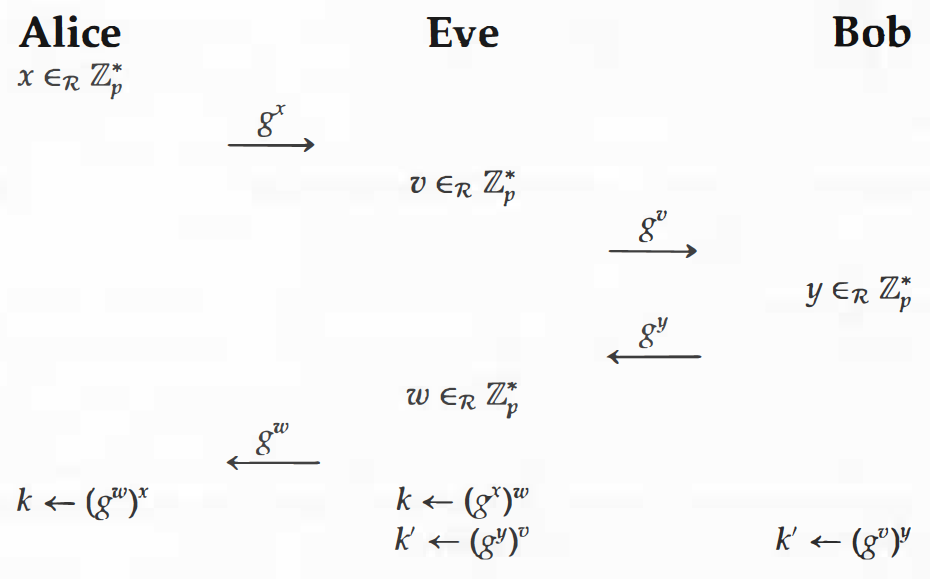
\includegraphics[scale=.5]{IMG/mitm}
\vspace{5mm}
\caption{\scriptsize Diagram from \emph{Cryptography Engineering} by Schneier, Ferguson, Kohno}
\end{figure}
\end{frame}


\begin{frame}
\frametitle{Digital Signatures}

A \textbf{digital signature} can be used to protect against the Man-In-The-Middle attack, to be discussed later in the course. 
\end{frame}

\begin{frame}
\frametitle{Next Class}

Next class we will discuss implementation of Diffie-Hellman.
\end{frame}

\begin{frame}
\frametitle{References}

\begin{itemize}
\item \emph{Cryptography Engineering} by Schneier, Ferguson, Kohno, Chapter 11
\end{itemize}
\end{frame}
\end{document}


